%===================  Dokument Typ  ========================
\documentclass[parskip,12pt,paper=a4]{scrartcl}
%\documentclass[parskip,12pt,paper=a4]{scrreprt}
%=================== Grundpakete Mathematik, Layout, Deutsche Zeichen ==============
\usepackage{amsmath, amssymb, graphics, setspace,amsthm}

\usepackage[left=3cm,right=3cm,top=3cm,bottom=3cm,includeheadfoot]{geometry}
\usepackage[ngerman]{babel}
\usepackage[utf8]{inputenc}
\usepackage[right]{eurosym}
\usepackage{enumerate}
\date{}
%================== BiBliographie ===============================================
\usepackage{cite}
\usepackage{bibgerm}


%========================= Blindtexte Einfügen  =============================================
\usepackage[]{blindtext}

%================== Überschriften Tabellen und Diagramme ========================
\usepackage{caption}
\usepackage{array}


\usepackage{graphicx}
\usepackage{lastpage}
\usepackage{longtable}

\usepackage[right]{eurosym}
\newcommand{\mathsym}[1]{{}}
\newcommand{\unicode}[1]{{}}

\setcounter{secnumdepth}{4}
\setcounter{tocdepth}{4}
\setcounter{section}{0}

% ===================== Colorierung von Tabellen   =================================
\usepackage{color}
\usepackage{colortbl}
\usepackage[table]{xcolor}

\definecolor{cell}{RGB}{220,230,240}
\definecolor{line}{RGB}{80,130,190}


\usepackage[T1]{fontenc}
\renewcommand{\familydefault}{\sfdefault}
\usepackage[]{helvet}
\usepackage[]{lastpage}
\usepackage[]{booktabs}
%\usepackage[]{scrpage2}
\usepackage{hyperref}
\usepackage{tabularx}
\usepackage{listings}
\usepackage{mdframed}
%==================== Definitionen und Sätze ===============================================

\newtheorem{mydef}{Definition}[section]
\newtheorem{mytheorem}{Satz}[section]
\newtheorem{myexample}{Beispiel}[section]
\newtheorem{myremark}{Bemerkung}[section]

%========================= Blindtexte Einfügen  =============================================
\usepackage[]{blindtext}
%====================== Kop- und Fußzeilen definieren  ================================
\usepackage{fancyhdr}
\pagestyle{fancy} %eigener Seitenstil
\fancyhf{} %alle Kopf- und Fußzeilenfelder bereinigen
\fancyhead[L]{} %Kopfzeile links
\fancyhead[C]{Praktikum Solvency II} %zentrierte Kopfzeile
\fancyhead[R]{ } %Kopfzeile rechts
\renewcommand{\headrulewidth}{2pt} %obere Trennlinie
\fancyfoot[L]{\tiny{\copyright Aktuarskanzlei Dr. Ströter\\Rüsselsheim, Oktober 2012}} %Fußzeile links
\fancyfoot[C]{Seite \thepage \ von\ \pageref{LastPage} } %Seitennummer
\fancyfoot[R]{Version 1.0} %Fußzeile rechts
\renewcommand{\footrulewidth}{1pt} %untere Trennlinie

\renewcommand{\headrule}{\vbox to 1pt{\hbox to\headwidth{\textcolor{blue}{\hrulefill}}\vss}} 
\renewcommand{\footrule}{\vbox to 0pt{\hbox to\headwidth{\textcolor{blue}{\hrulefill}}\vss}}



% Links Blau einfärben 
%\usepackage{hyperref}
%\hypersetup{%
%  colorlinks=true,   % color references
%  linkcolor = blue,  % Linkcolor blue
%  citecolor = blue,  % cite-color  blue
%  urlcolor = blue,  % cite-color blue
%  pdfpagemode=UseNone,  % PDF-Viewer startet ohne Inhaltsverzeichnis et.al.
%  pdfstartview=FitH} % PDF-Viewer benutzt beim Start bestimmte Seitenbreite
  
  
\begin{document}
\titlehead{Fachbereich Mathematik\\Johann Wolfgang Goethe Universität}
\title{Berechnung des SCR eines Modellversicherungsbestandes nach Maßgaben von Solvency II}
\subtitle{\textit{--------\\Praktikumsdokumentation\\zur\\ Vorlesung Solvency II}}
\author{Friedrich H. Schäufele, \\ Matr.Nr. 3674477}

\maketitle


\begin{abstract}
\noindent  
\end{abstract}
\clearpage
\tableofcontents
\clearpage


%%%%%%%%%%%%%%%%%%%%%%%%%%%%%%%%%%%%%%%%%%%%%%%%%%%%%%%
%%%%%%%%%%%%%%%%%%%%%%%%%%%%%%%%%%%%%%%%%%%%%%%%%%%%%%%
%%%%%%%%%%%%%%%%%%%%%%%%%%%%%%%%%%%%%%%%%%%%%%%%%%%%%%%
\section{Grundlagen}

%%%%%%%%%%%%%%%%%%%%%%%%%%%%%%%%%%%%%%%%%%%%%%%%%%%%%%%
\subsection{Aufgabenstellung}
Aus dem Modellbestand einer privaten Pflegeversicherung mit 34.884 Versicherten werden zuerst anhand der 
gegebenen Formeln die individuellen Versicherungsprämien der einzelnen Kunden ermittelt. Darauf aufbauend wird die Deckungsrückstellung des Versicherers berechnet. 
Nach Ermittlung der Prämien und der Deckungswertrückstellung werden anhand des implementierten Simulationsmodells
die Erwartungswertrückstellungen für verschiedene Standard- und Stresszenarien kalkuliert.
Abschließend wird die Solvenzbilanz mit dem entsprechenden Solvency Capital Requirement (SCR) erstellt.  
Das SCR soll sicherstellen, dass zu 99,5\% kein technischer Ruin der Versicherung eintritt.

Vorgegeben sind u.a. Werte für den Rechnungszins, Marktzinsen, Sterbewahrscheinlichkeiten, Stornowahrscheinlichkeiten, Eintrittswahrscheinlichkeiten der jeweiligen Pflegestufen, Kopfschäden sowie Werte für das Alter der Kunden und vereinbarte Leistungen.

Das Modell und die Simulationen werden in \textsc{R} implementiert und ausgeführt. Der Source-Code der Implementation ist in Auszügen im Anhang zu finden. 

%%%%%%%%%%%%%%%%%%%%%%%%%%%%%%%%%%%%%%%%%%%%%%%%%%%%%%%
\subsection{Beschreibung Modellversicherung}

Im Bestand der Versicherung befinden sich ca. 35.000 Versicherte mit einem Durchschnittsalter von ca. 47 Jahren. Die Versicherten weisen eine Mitgliedsdauer zwischen null und vier Jahren auf und sind jeweils zur Hälfte männlich bzw. weiblich.
Bei Eintritt eines Pflegfalls wird in Pflegestufe I monatlich 40\%, in Pflegestufe II monatlich 70\% und in Pflegestufe III 
monatlich 100\% der individuell festgelegten Leistung ausgezahlt. \\


%%%%%%%%%%%%%%%%%%%%%%%%%%%%%%%%%%%%%%%%%%%%%%%%%%%%%%%
\subsection{Vorgaben durch Solvency II}
Die Solvenzkapitalanforderung (SCR) entspricht dem \glqq Value-at-Risk (VaR) der Basiseigenmittel zu einem Konfidenzniveau von 99,5\% über den Zeitraum eines Jahres\grqq .

Der VaR ist definiert als die kleinste Zahl, für die gilt
\begin{align*}
99,5\% \le P(\Delta BEM \le VaR)
\end{align*}

und in unserem Fall gilt vereinfacht 
\begin{align*}
VaR = SCR = BSCR
\end{align*}

mit
\begin{align*}
BSCR = \sqrt{ \sum_{i,j} CORR_{i,j} * SCR_i * SCR_j }.
\end{align*}

%%%%%%%%%%%%%%%%%%%%%%%%%%%%%%%%%%%%%%%%%%%%%%%%%%%%%%%
%%%%%%%%%%%%%%%%%%%%%%%%%%%%%%%%%%%%%%%%%%%%%%%%%%%%%%%
\section{Simulation}

%%%%%%%%%%%%%%%%%%%%%%%%%%%%%%%%%%%%%%%%%%%%%%%%%%%%%%%
\subsection{Bestimmung der Beiträge sowie des Deckungskapitals des Bestandes}

Zur Bestimmung der monatlichen Beiträge der einzelnen Versicherungsnehmer werden die in der Praktikumsaufgabe
gegebenen Formeln sowie das Äquivalenzprinzip angewendet.

Darauf aufbauend wird das Deckungskapitals in zwei verschiedenen Szenarien berechnet. Während {\itshape Rechnungszinsszenario A} einen konstanten Rechnungszins von 2\% über die komplette Simulationszeit verwendet, wird in {\itshape Rechnungszinsszenario B} der Rechnungszins nach 5 Jahren von 2\% auf 1,5\% gesenkt.

\begin{table}[h!]
  \centering
  \label{table1}
  \begin{tabular}{|c|c|}
	\hline
    	Zinsszenario A & Zinsszenario B\\
    	\hline
    	74.354.339 & 81.819.031 \\
	\hline
  \end{tabular}
\caption{Ergebnisse der Berechnung des Deckungskapitals}
\end{table}

Anhand dieser Vorgaben wurde für das Rechnungszinsszenario A ein Wert von $74,4$ Mio. Euro und für das Zinsszenario B ein Wert von $81,8$ Mio. Euro ermittelt (siehe Tabelle)

\subsection{Simulationsszenarien gemäß gegebener Standardformel}

Die Ermittlung der jeweiligen Erwartungswertrückstellung bzw. des jeweiligen SCR wurde für alle gegebenen Zinszenarien sowie für das \glqq Langlebigkeitsszenario\grqq \ und das \glqq Stornoszenario\grqq \ durchgeführt. Hierfür wurden die gegebenen Formeln aus der Vorlesung verwendet. Die ermittelten Werte sind in {\itshape 2.3 Ergebnisse} zu finden.

Generell lässt sich sagen, dass ich mit den ermittelten Ergebnissen zufrieden bin und diese den Voraussetzungen entsprechend in die \glqq richtige Richtung laufen\grqq . Wie erwartet verringert bzw. erhöht sich die Rückstellung bei steigenden bzw. fallenden Zinsen aufgrund des jeweiligen Diskontierungfaktors, Langlebigkeit erhöht und Massenaustritte verringert die Rückstellung. 

Enttäuschend war jedoch die relativ lange Laufzeit einer einzelnen Simulation (ca. 105 sec pro Simulation).
Aufgrund der langen Laufzeit wurden anstatt der gewünschten 1000 Simulationen pro Zinsszenario nur 23 Simulationen sowie für die beiden Szenarien der Langlebigkeit und des Massenstornos jeweils nur 15 Simulationen durchgeführt. Dies mag zwar wenig zu den geforderten 1000 erscheinen, lässt sich aber mit den gegebenen Mitteln nicht zeitgerecht erfüllen. Daher wurde in diesem Fall nicht die Normalverteilung sondern die Student-Verteilung bei der Bestimmung des Konfidenzintervalls verwendet. Dadurch wird das Konfidenzintervall etwas breiter, was sich in einem etwas höheren SCR bzw. VaR niederschlagen sollte.

\subsubsection{Grundlegendes zu den Simulationen}
Angenommen wird, dass bei Stornierung des Versicherungsvertrages, wie in der Realität üblich, die gesamten eingezahlten Mittel im Jahr der Stornierung komplett ausbezahlt werden. Da sich die Stornierungen in den Zinsszenarien in Grenzen halten hat dieser Umstand relativ geringe Auswirkungen auf die jeweilige Erwartungswertrückstellung.

\subsubsection{Standardszenario}
Das Standardszenario diskontiert die anfallenden Cashflows mit den am Markt vorherrschenden Zinsen für die jeweilige Laufzeit.
 
\subsubsection{Szenario Zinsschocks}
Wie erwartet lässt ein niedriges Zinsumfeld (Shockdown-Szenarien) die Erwartungswertrückstellungen in die Höhe schnellen. Andererseits verringern hohe Zinsen die Rückstellung in hohem Maße.

\subsubsection{Szenario Langlebigkeit}
Das Langlebigkeitsszenario erhöht das in den Simulationen durchschnittliche erreichbare Alter um ca. 2 Jahre. Dieser Effekt schlägt sich direkt in einer stark steigenden Erwartungswertrückstellung nieder.  

\subsubsection{Szenario StornoShok}
Angenommen wird, dass in 5 Jahren 50\% der Kunden den Versicherungsvertrag kündigen. Da somit der Betrag der zukünftigen Cashflows stark verringert wird reduziert sich infolge dessen auch die Erwartungswertrückstellung.

\newpage
\subsection{Ergebnisse}

Die Ergebnisse der Simulationen sind in der folgenden Tabelle aufgelistet:

\begin{table}[h!]
  \centering
  \label{table1}
  \begin{tabular}{|c|c|}
	\hline
    	Szenario $i$ & ermittelte $SCR_i$ in Euro \\
    	\hline
    	Basisszenario (RFNoVA) & 1.236.497.182 \\        
	\hline
    	RFVA & 1.144.021.540 \\
	\hline
    	NShockUP & 892.795.200 \\
	\hline
    	NShockDown & 1.492.683.319    \\
	\hline
    	VShockUp &  832.030.693 \\
	\hline
    	VShockDown & 1.393.195.783 \\
	\hline
    	Langlebigkeit &  1.360.298.501\\
	\hline
    	Storno & 651.623.154 \\
	\hline
  \end{tabular}
\caption{Ergebnisse der Berechnung des Deckungskapitals}
\end{table}

In folgender Abbildung sind die Ergebnisse der jeweiligen Simulationen graphisch dargestellt:
\begin{figure}[h]
\centering
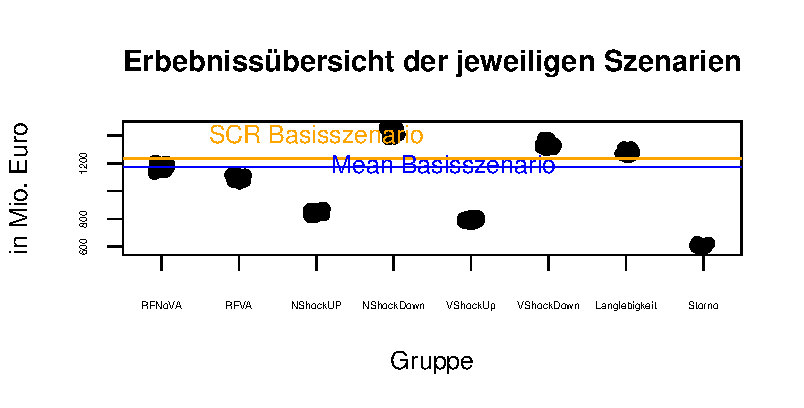
\includegraphics[scale=1.2]{Gesamtplot_1.pdf}
\caption{Simulationsergebnisse, siehe Anhang}
\end{figure}

Es lässt sich erkennen dass sich die verschiedenen Szenarien teilweise deutlich voneinander unterscheiden und dass die Streuung in den einzelnen Gruppen relativ niedrig ist.

\section{Erstellung einer Solvenzbilanz}

Wie in {\itshape Solvabilitätsvorschriften für Krankenversicherer} gegeben lässt sich in unserem vereinfachten Modell der VaR bzw. SCR folgendermaßen berechnen:
\begin{align*}
VaR = SCR = BSCR = \sqrt{\sum_{i,j} Corr_{i,j} SCR_i SCR_j}
\end{align*}

Der VaR wird nun für das Basisszenario (RFNoVA) sowie Langlebigkeits- und Stornoszenario berechnet. Korrelationskoeffizienten sind meiner Kenntnis nach nur für das Langlebigkeits- und Stornoszenario gegeben. Daher werden die weiteren Korrelationskoeffizienten Null bzw. Eins gesetzt. Die Berechnung ergibt einen 
\begin{align*}
VaR = 2.060.861.720 \  Euro,
\end{align*}
was auch dem Endergebnis dieser Arbeit entspricht.

\section{Auszüge Code}

Auszüge aus dem Code, hier insbesondere aus dem Algorithmus der Simulation:
\begin{tiny}
\lstset{language=R, keywordstyle=\color{blue}, commentstyle=\color{black},}
\begin{mdframed}
\begin{lstlisting}

Bestand <- read.csv("Bestand.csv", header = TRUE)
Tafeln <- read.csv("TafelnAktualisiert.csv", header = TRUE)
Zinsstrukturkurven <- read.csv("Zinsstrukturkurven.csv", header = TRUE)

### Variablen

# maximal erreichbares Alter
AgeMax = length(Tafeln$x)

# Option Langlebigkeit
langesLeben = FALSE

# Option Massenstorno
Massenaustritt = FALSE
MassenaustrittImJahr = 5
MassenaustrittsRate = 0.5

### erstelle und lese Abzinsungstabelle ein

source('Projekt_abzinsungstabellen.R',local = TRUE)

### lese Arbeitsschritt 1 ein - Funktionen und Ausgabe fuer tPx

source('Projekt_Arbeitsschritt_1.R',local = TRUE)
#create tPx Matrix with specific lambdas
tPx_gesamt_Matrix <- create_tPx_gesamt_Matrix(1,1)

### lese Arbeitsschritt 2 ein - Funktionen und Ausgabe fuer tVx

source('Projekt_Arbeitsschritt_2.R',local = TRUE)

Deckungsrueckstellung = sum(t_V_x_einzeln_vec)

Deckungsrueckstellung_einnahmen_seit_Versicherungsbeginn = P_x_PST_einzeln_vec
for (i in 1:length(Deckungsrueckstellung_einnahmen_seit_Versicherungsbeginn)) {
  Deckungsrueckstellung_einnahmen_seit_Versicherungsbeginn[i] =
 Deckungsrueckstellung_einnahmen_seit_Versicherungsbeginn[i]*Bestand$t[i]
}
sum(Deckungsrueckstellung_einnahmen_seit_Versicherungsbeginn)
#write(sum(Deckungsrueckstellung_einnahmen_seit_Versicherungsbeginn), file = 
"Deckunsrueckstellung_konstZins.csv", sep = ',')

### Simulation - Vorbereitungen und Start
### Arbeitsschritt 3 und 4

# Anzahl Simulationen
n = 23

# EWR-Matrix zum abspeichern der berrechneten EWR-Werte
# EWR_vec = matrix(nrow = 1,ncol=n,byrow=TRUE)
#EWR_vec = rep(0,6*n)
#EWR_group_vec = rep(0,6*n)
EWR_vec = rep(0,n)
EWR_group_vec = rep(1,n)


system.time(
# starte berechnungen
for (p in 1:(n)) {
  # baue Eintrittstabelle mit Werten fuer Eintritt in die jeweilige Pflegestufe und Sterbealter
  # Eintrittstabelle <- matrix(nrow = 4,ncol=length(Bestand$x),byrow=TRUE)
  Eintrittstabelle <-
    matrix(nrow = 5,
           ncol = length(Bestand$x),
           byrow = TRUE)
  # rownames(Eintrittstabelle) <- c('clientDiesAt','clientInPST3At','clientInPST2At','clientInPST1At')
  rownames(Eintrittstabelle) <-
    c('clientDiesAt',
      'clientInPST3At',
      'clientInPST2At',
      'clientInPST1At',
      'StornoAt')
  #countAustritt = 0
  # Algoritmus fuer das Befuellen der Eintrittstabelle
  for (i in 1:ncol(Eintrittstabelle)) {
    Eintrittstabelle[1, i] = AgeMax
    Eintrittstabelle[2, i] = AgeMax + 1
    Eintrittstabelle[3, i] = AgeMax + 1
    Eintrittstabelle[4, i] = AgeMax + 1
    Eintrittstabelle[5, i] = AgeMax + 1

    for (j in (Bestand$x[i] + Bestand$t[i]):AgeMax) {
      if (langesLeben == FALSE && runif(1, 0, 1) <= Tafeln$qx_m[j]) {
        Eintrittstabelle[1, i] = j
        break
      }
      if (langesLeben == TRUE && runif(1, 0, 1) <= Tafeln$qx_m[j]*0.8) {
        Eintrittstabelle[1, i] = j
        break
      }
      if (runif(1, 0, 1) <= Tafeln$Px_III[j]) {
        Eintrittstabelle[2, i] = j
      }
      if (runif(1, 0, 1) <= Tafeln$Px_II[j] &&
          j < Eintrittstabelle[2, i]) {
        Eintrittstabelle[3, i] = j
      }
      if (runif(1, 0, 1) <= Tafeln$Px_I[j] &&
          j < Eintrittstabelle[2, i] && j < Eintrittstabelle[3, i]) {
        Eintrittstabelle[4, i] = j
      }
      if (Massenaustritt == FALSE && runif(1, 0, 1) <= Tafeln$wx_m[j] &&
          j < Eintrittstabelle[2, i] &&
          j < Eintrittstabelle[3, i] && j < Eintrittstabelle[4, i]) {
        Eintrittstabelle[5, i] = j
      }
      if (Massenaustritt == TRUE) {
        Austritt = FALSE
        if (j == (Bestand$x[i] + Bestand$t[i]) && runif(1,0,1) < MassenaustrittsRate) {
          Austritt = TRUE
          #countAustritt = countAustritt+1
          Eintrittstabelle[5, i] = Bestand$x[i] + Bestand$t[i] + MassenaustrittImJahr
        }
        if (Austritt == FALSE && runif(1, 0, 1) <= Tafeln$wx_m[j] &&
            j < Eintrittstabelle[2, i] &&
            j < Eintrittstabelle[3, i] && j < Eintrittstabelle[4, i]) {
          Eintrittstabelle[5, i] = j
        }
      }
    }
  }
  
  ### Erwartungswert berechnen
  # EWR = E[SUM_{j=0}^{w}(Ausgaben - Einnahmen)*(Abzinsungsfaktor)]
  # Ausgaben = Sum(q*L)
  # q = 1, 0.7, 0.4 je nach Pflegestufe
  # w = todesalter oder storno
  # berechne Ausgaben/Einnahmen pro Klienten und fasse am Schluss zusammen
  
  EWR = 0
  
  # setze diskontfaktor
  ZinsSK = 1
  # if (p<=n) {
  #   ZinsSK = 1
  #   EWR_group_vec[p] = 1
  # }
  # if (p>n && p<=2*n) {
  #   ZinsSK = 2
  #   EWR_group_vec[p] = 2
  # }
  # if (p>2*n && p<=3*n) {
  #   ZinsSK = 3
  #   EWR_group_vec[p] = 3
  # }
  # if (p>3*n && p<=4*n) {
  #   ZinsSK = 4
  #   EWR_group_vec[p] = 4
  # }
  # if (p>4*n && p<=5*n) {
  #   ZinsSK = 5
  #   EWR_group_vec[p] = 5
  # }
  # if (p>5*n) {
  #   ZinsSK = 6
  #   EWR_group_vec[p] = 6
  # }
  
  for (i in 1:ncol(Eintrittstabelle)) {
    # aktuelles alter
    actAge = Bestand$x[i] + Bestand$t[i]
    
    # buffer fuer storno
    storno = FALSE
    
    # berechne w = Alter bei dem Ein- und Auszahlungen enden
    endAge = Eintrittstabelle[1, i]
    if (Eintrittstabelle[5, i] < Eintrittstabelle[1, i]) {
      endAge = Eintrittstabelle[5, i]
      storno = TRUE
    }
    
    # years to maturity
    w = endAge - actAge
    
    #cat('w = ')
    #cat(w)
    #cat('\n')
    
    
    # erstelle vektor q fuer schadenklasse
    if (w > 0) {
      q_vec <- rep(0,w)
      p_vec <- rep(1,w)
    }
    else{
      q_vec = 0
      p_vec = 0
    }
    
    if (storno == TRUE) {
      q_vec[w] = (w-1)*P_x_PST_einzeln_vec[i]
      p_vec[w] = 0.0
    }
    
    # years to pstI
    ytPST1 = Eintrittstabelle[4, i] - actAge
    if (ytPST1 < w && storno == FALSE) {
      for (k in 1:(w - ytPST1)) {
        q_vec[ytPST1 + k] = 0.4
        p_vec[ytPST1 + k] = 0.0
      }
    }
        
    # years to pstII
    ytPST2 = Eintrittstabelle[3, i] - actAge
    if (ytPST2 < w && storno == FALSE) {
      for (k in 1:(w - ytPST2)) {
        q_vec[ytPST2 + k] = 0.7
        p_vec[ytPST2 + k] = 0.0
      }
    }    
    
    # years to pst3
    ytPST3 = Eintrittstabelle[2, i] - actAge
    if (ytPST3 < w && storno == FALSE) {
      for (k in 1:(w - ytPST3)) {
        q_vec[ytPST3 + k] = 1
        p_vec[ytPST3 + k] = 0.0
      }
    }
    
    for (k in 1:length(q_vec)) {
      if (k <= ncol(DiskontZinsTabelle)) {
        q_vec[k] = q_vec[k] * DiskontZinsTabelle[ZinsSK, k]
        p_vec[k] = p_vec[k] * P_x_PST_einzeln_vec[i]*DiskontZinsTabelle[ZinsSK,k]
      }
      if (k > ncol(DiskontZinsTabelle)) {
        q_vec[k] = q_vec[k] * DiskontZinsTabelle[ZinsSK, ncol(DiskontZinsTabelle)]
        p_vec[k] = P_x_PST_einzeln_vec[i]*DiskontZinsTabelle[ZinsSK,ncol(DiskontZinsTabelle)]
      }
    }

    if (storno == TRUE) {
      EWR = EWR + sum(q_vec) - sum(p_vec)
    }
    if (storno == FALSE) {
      EWR = EWR + 12 * Bestand$L[i] * sum(q_vec) - sum(p_vec)
    }
  }
  EWR_vec[p] = EWR
})

results_vec <- c(EWR_vec,EWR_group_vec)
\end{lstlisting}
\end{mdframed}
\end{tiny}

\end{document}





